\section{Results}
\label{sec:Res}

% ----------------------------------------------------------------------- %
% ----------------------------------------------------------------------- %
\subsection{General estimation results}
\label{sec:feasest}

An application of the SRS, \psmall{} and \extpsynth{} estimator was not feasible for 17 of all 405 FR-units due to an insufficient terrestrial sample size of $n_{2,G} < 2$. We further restricted the calculation of \psmall{} and \extpsynth{} to small area units with a minimum terrestrial sample size of $n_{2,G} \geq 4$ to avoid unstable estimates. This affected 65 additional FR units and limited unbiased two-phase estimations to 321 (79\%) of the 405 FR units. It should be noted that also the \psynth{} estimator could not be applied for 2 FR-units since $n_{1,G} < 1$. Due to substantial larger sample sizes, all estimators could however be applied in all small area units on the FA level. The average value and the range of the mean timber volume estimates over the evaluated FA and FR units turned out to be very similar between all estimators (table \ref{tab:estres}). An additional pairwise comparison of the 95\% confidence intervals for all FA- and FR-units revealed that the four estimators did in fact not produce statistically different point estimates. This confirmed that the differences between the estimators are solely found in the precision which they provide for the point estimates.


%% NOTES
%
% Feasibility: 
% FA-level: for 44 out of 45 FA-units, the full model could be applied. For one remaining, only the model without tree species was applied.
% 
% FR-level: 
% o mathemat. feasibility:
%    - op-estimation feasible for 388 of the 405 fu-units. --> for 17 fus not possible due to n2G < 2
%    - psmall / extpsynth possible for 388 of the 405 units (for 17 fus not possible). Reason: n2G < 2 (identical with op)
%    - psynth not possible for 403 of 405. For 2 units not possible due to n1G < 2 (these two are included in the 19 above).
%    -> basically, for these 2 fu-units, none of the estimators could produce estimations due to n1G < 2
%  o restriction of unbiased estimtors to n2G >= 4: 
%    - psmall / extpsynth: 65 of the 386 fu-units have n2G < 4, so theyx cancel out. Thus we have 19 + 65 = 84 fu-units for which no psmall & extpsynth estimations were deliverable.
%       ==> Thus, we have unbiase estimations for 321 of 405 fu units (79%)

% Mention: a comparison of the confidence intervals between revealed that the 

\begin{table}[H]
	\begin{center}
		\caption{Descriptive summary of point estimates and estimation errors on the two forest district levels. $N_u$: number of evaluated small area units.}
		\vspace{0.2cm}
		\label{tab:estres}
		{\small %
			\begin{tabular}{c|l c|c|c|c|c|c|c} %8cols
				\hlineB{1}
				\multirow{2}{*}{District level} & \multicolumn{2}{c|}{\multirow{2}{*}{Estimator}} & \multicolumn{3}{c|}{Point estimates} & \multicolumn{3}{c}{Errors [\%]} \\
				\cline{4-9} & & & mean & min & max & mean & min & max \\
				\hline \hline
				\multirow{4}{*}{FA} & SRS       & ($N_u$=45)  & 300.16 & 215.91 & 392.84 &  6.69 & 3.87 & 13.21 \\
				                    & PSMALL    & ($N_u$=45)  & 307.29 & 209.26 & 417.10 &  5.16 & 3.46 & 14.33 \\
				                    & EXTPSYNTH & ($N_u$=45)  & 307.27 & 209.01 & 415.02 &  4.78 & 3.25 & 13.88 \\
				                    & PSYNTH    & ($N_u$=45)  & 306.90 & 223.51 & 409.92 &  2.34 & 1.54 &  3.95 \\
				\hlineB{2}          
				\multirow{4}{*}{FR} & SRS       & ($N_u$=388) & 301.83 &  99.89 & 612.13 & 18.32 & 0.34 & 104.97 \\
				                    & PSMALL    & ($N_u$=321) & 308.15 & 159.64 & 568.67 & 12.24 & 3.48 &  44.94 \\
				                    & EXTPSYNTH & ($N_u$=321) & 308.38 & 154.07 & 544.34 & 11.34 & 3.60 &  40.91 \\
				                    & PSYNTH    & ($N_u$=403) & 307.82 & 166.01 & 444.29 & 4.65  & 2.56 &  62.51 \\
				\hline \hline
			\end{tabular}
		}%
	\end{center}
\end{table}



% ----------------------------------------------------------------------- %
% ----------------------------------------------------------------------- %
\subsection{Estimation errors}
\label{sec:esterr}

On both small area levels, the design-unbiased estimators \psmall{} and \extpsynth{} led to a substantial reduction in the estimation errors compared to the SRS estimator (fig. \ref{fig:disterrors}). On the FA level, the SRS estimator yielded an estimation error of 6.7\% on average compared to 5.2\% and 4.8\% under the \extpsynth{} and \psmall{} estimator (table \ref{tab:estres}). The cumulative error distribution (fig. \ref{fig:disterrors}, left) reveals that under the SRS estimator, errors $\leq$ 5\% were achieved for 17\% of the FA units (8 of 45). This proportion could be increased to 62\% (28 FA units) and 73\% (33 FA units) by application of \psmall{} and \extpsynth{}. 95\% of all estimates exhibited errors $\leq$ 9.5\% under the SRS estimator and $\leq$ 6.6\% when using \psmall{} or \extpsynth{}. Estimation errors higher than 10\% only appeared twice for each of the unbiased estimators.\par
The error reduction by the unbiased double sampling estimators was even more pronounced on the FR level (fig. \ref{fig:disterrors}, right), although the overall error niveau was substantially higher than on FA level. The average error under the SRS estimator was 18.3\%, while it was 11.3\% and 12.2\% under the \psmall{} and \extpsynth{} estimator (table \ref{tab:estres}). Errors smaller than 10\% were achieved in 15\% by the SRS estimator and 46\% by the \psmall{} and \psynth{} estimator. 95\% of the 321 FR units where \psmall{} and \extpsynth{} could be applied exhibited errors $\leq$ 20\%. In comparion, the SRS estimates resulted in errors $\leq$ 36.6\% for 95\% of the 388 FR units.

\begin{figure}[H]
	\centering
	\resizebox{1\hsize}{!}{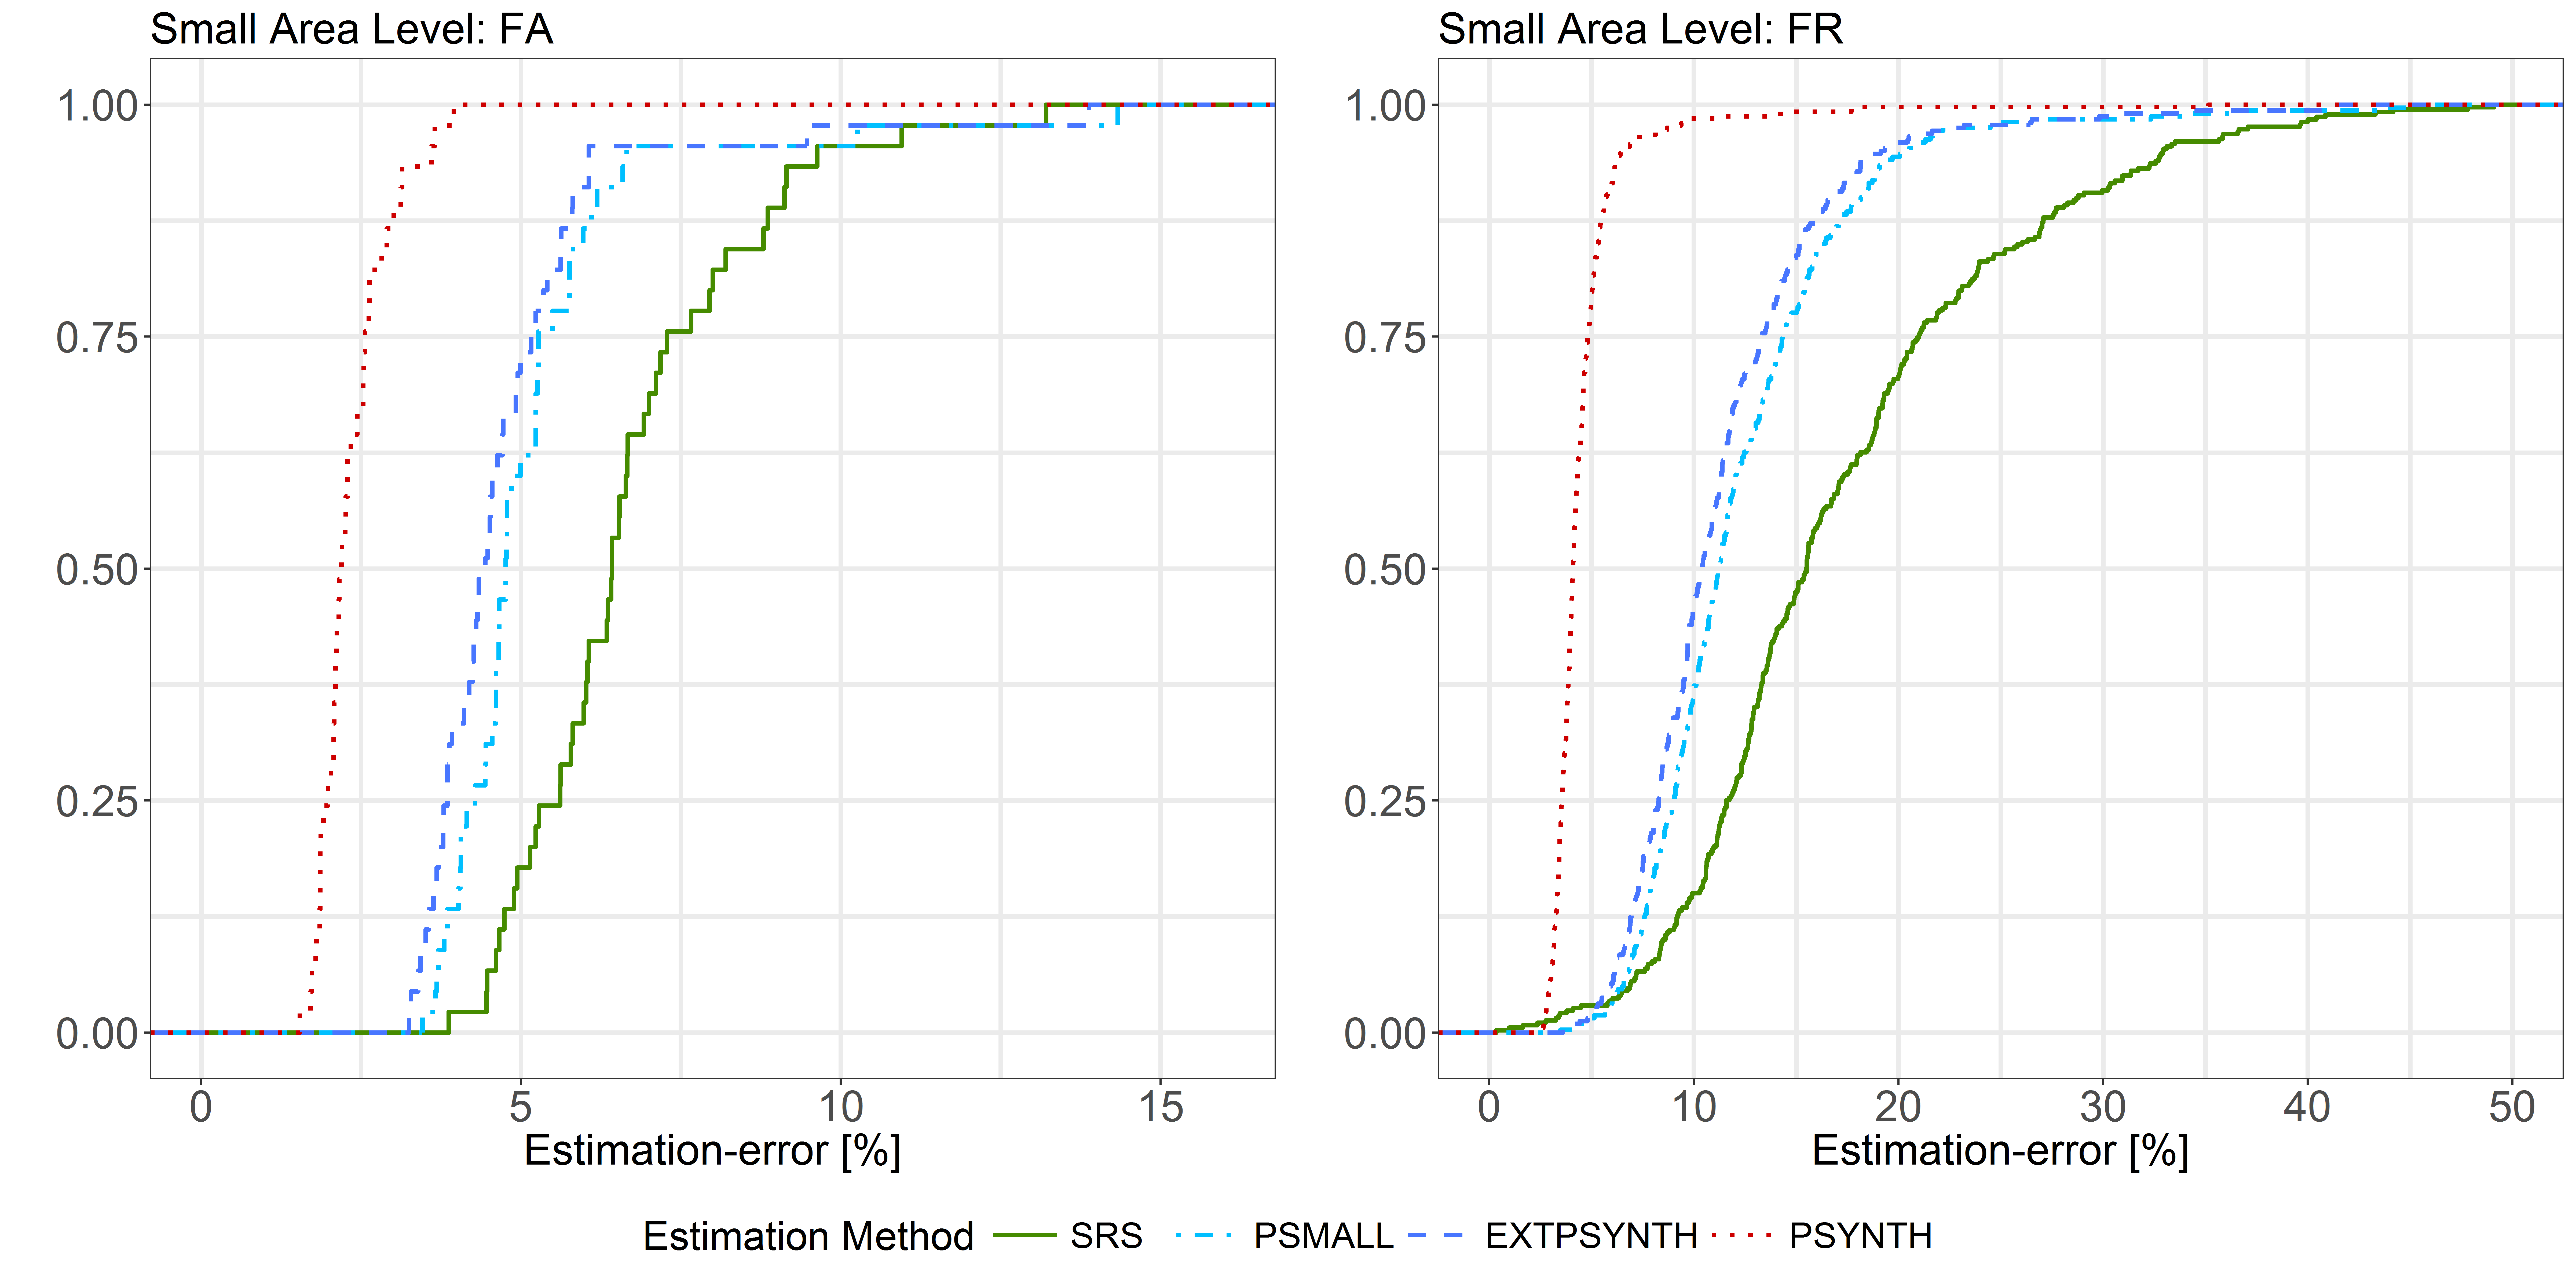
\includegraphics{fig/error_distr_foa_fu.png}}
	\caption{Cumulative distribution of estimation errors under the simple random sampling (SRS), the pseudo small (\psmall{}), the extended pseudo synthetic (\extpsynth{}) and the pseudo synthetic (\psynth{}) estimator. \textit{Left}: Results for the 45 FA units. \textit{Right}: Results for the 388 (SRS), 321 (\psmall{} / \extpsynth{}) and 403 (\psynth{}) FR units.}
	\label{fig:disterrors}
\end{figure}

On both small area levels, the \psynth{} estimator resulted in much smaller estimation errors compared to \psmall{} and \extpsynth{}. This was as expected, since the \psynth{} variance estimate does not take the residual variation in each small area unit into account (section \ref{sec:psynth}). Compared to the error distribution of the asymptotically design-unbiased estimators \psmall{} and \extpsynth{}, the estimation errors of \psynth{} might thus be to optimistic.

%% NOTES
 %Estimation errors smaller than 10\% were achieved for only 15\% (xx) of all FR units under SRS, while this proportion could be increased to 38\% and 46\% by PSMALL and EXTPSYNTH. 




% ----------------------------------------------------------------------- %
% ----------------------------------------------------------------------- %
\subsection{Comparison of \psmall{} and \extpsynth{}}
\label{sec:comp}

Figure \ref{fig:disterrors} revealed that the error distribution of \psmall{} and \extpsynth{} are very similar, with \psmall{} showing marginally higher estimation errors. In order to investigate the differences between \psmall{} and \extpsynth{}, we compared the g-weight variances of both estimators for all 321 FR units (fig. \ref{fig:compvar}, left). As obvious, \psmall{} yielded slightly larger variances for the vast majority of the estimates. As addressed in section \ref{sec:extpsynth}, one possible explanation for such differences was the effect of one or more cluster not entirely being included in a small area unit, as this would constitute a violation of the \extpsynth{} estimator. This violation was actually observed in 155 of the 321 FR units (48\%). However, the affected FR units (depicted in red color, fig. \ref{fig:compvar}) did not show a significant divergence from the \psmall{} variances with respect to the remaining unaffected FR units. The variance differences between the two estimators were expected to occur for the following reason: as depicted in \citet[pp.17--18]{mandallaz2016}, the mathematical formulations of the \psmall{} and \extpsynth{} estimator are asymptotically equivalent only under large terrestrial sample sizes $n_{2,G}$ within the small area. An additional comparison of the absolute differences in the g-weight variance (fig. \ref{fig:compvar}, right) revealed that large differences did in fact particularly occur for small area units with small terrestrial sample sizes ($n_{2,G} \leq 5$). The differences decreased with increasing sample size and thus confirmed the asymptotic relationship between the two estimators. However, a comparison of the confidence intervals of \psmall{} and \extpsynth{} revealed that the variance differences did not lead to statistically significant point estimates.\par


% NOTES:
% - Section \ref{sec:comp} provides a more detailed analysis of the differences between the two estimators.
% - DM-explanation: The model residuals and thus the residual variance for extpsynth should in general be a bit better than those of psmall, since we additionally adjust the regression
%                   to the small area data by introducing the sae-indicator variable (even if this is strictly speaken only a means to cause zero-mean-residuals)
%                   ==> we even can relate the differences to the residual variation, since the first and second term of extpsynth and psmall area identical with exception 
%                       of the adjusted regression coefficient
% - we can see the asymptotic of psmall and extpsynth: with increasing n2G, psmall and extpsynth are mathematically identical
% ==> so differences will particularly concern sae units with small n2G (threshold seems to be around n2G < 10)
%
% for Discussion:
% - our analyses 
%   a) suggest that the differences between \psmall{} and \extpsynth{} become negligible for sample sizes $n_{2,G}$ larger than 10 due to the asymptotic relationship between these estimators 
%   b) showed that violation of the '\extpsynth{}'-assumption had only minor effects on the variance estimates that did not lead to statistically different point estimates 
%   c) indicate that \extpsynth{} will in general have slightly smaller est.variances due to a slightly better model fit through the data in the small area, which is caused by the 
%      adjusted intercept (which however is mainly a means to insure the zero-mean-residual assumption in the \extpsynth{}-estimator


\begin{figure}[H]
	\centering
	\resizebox{1\hsize}{!}{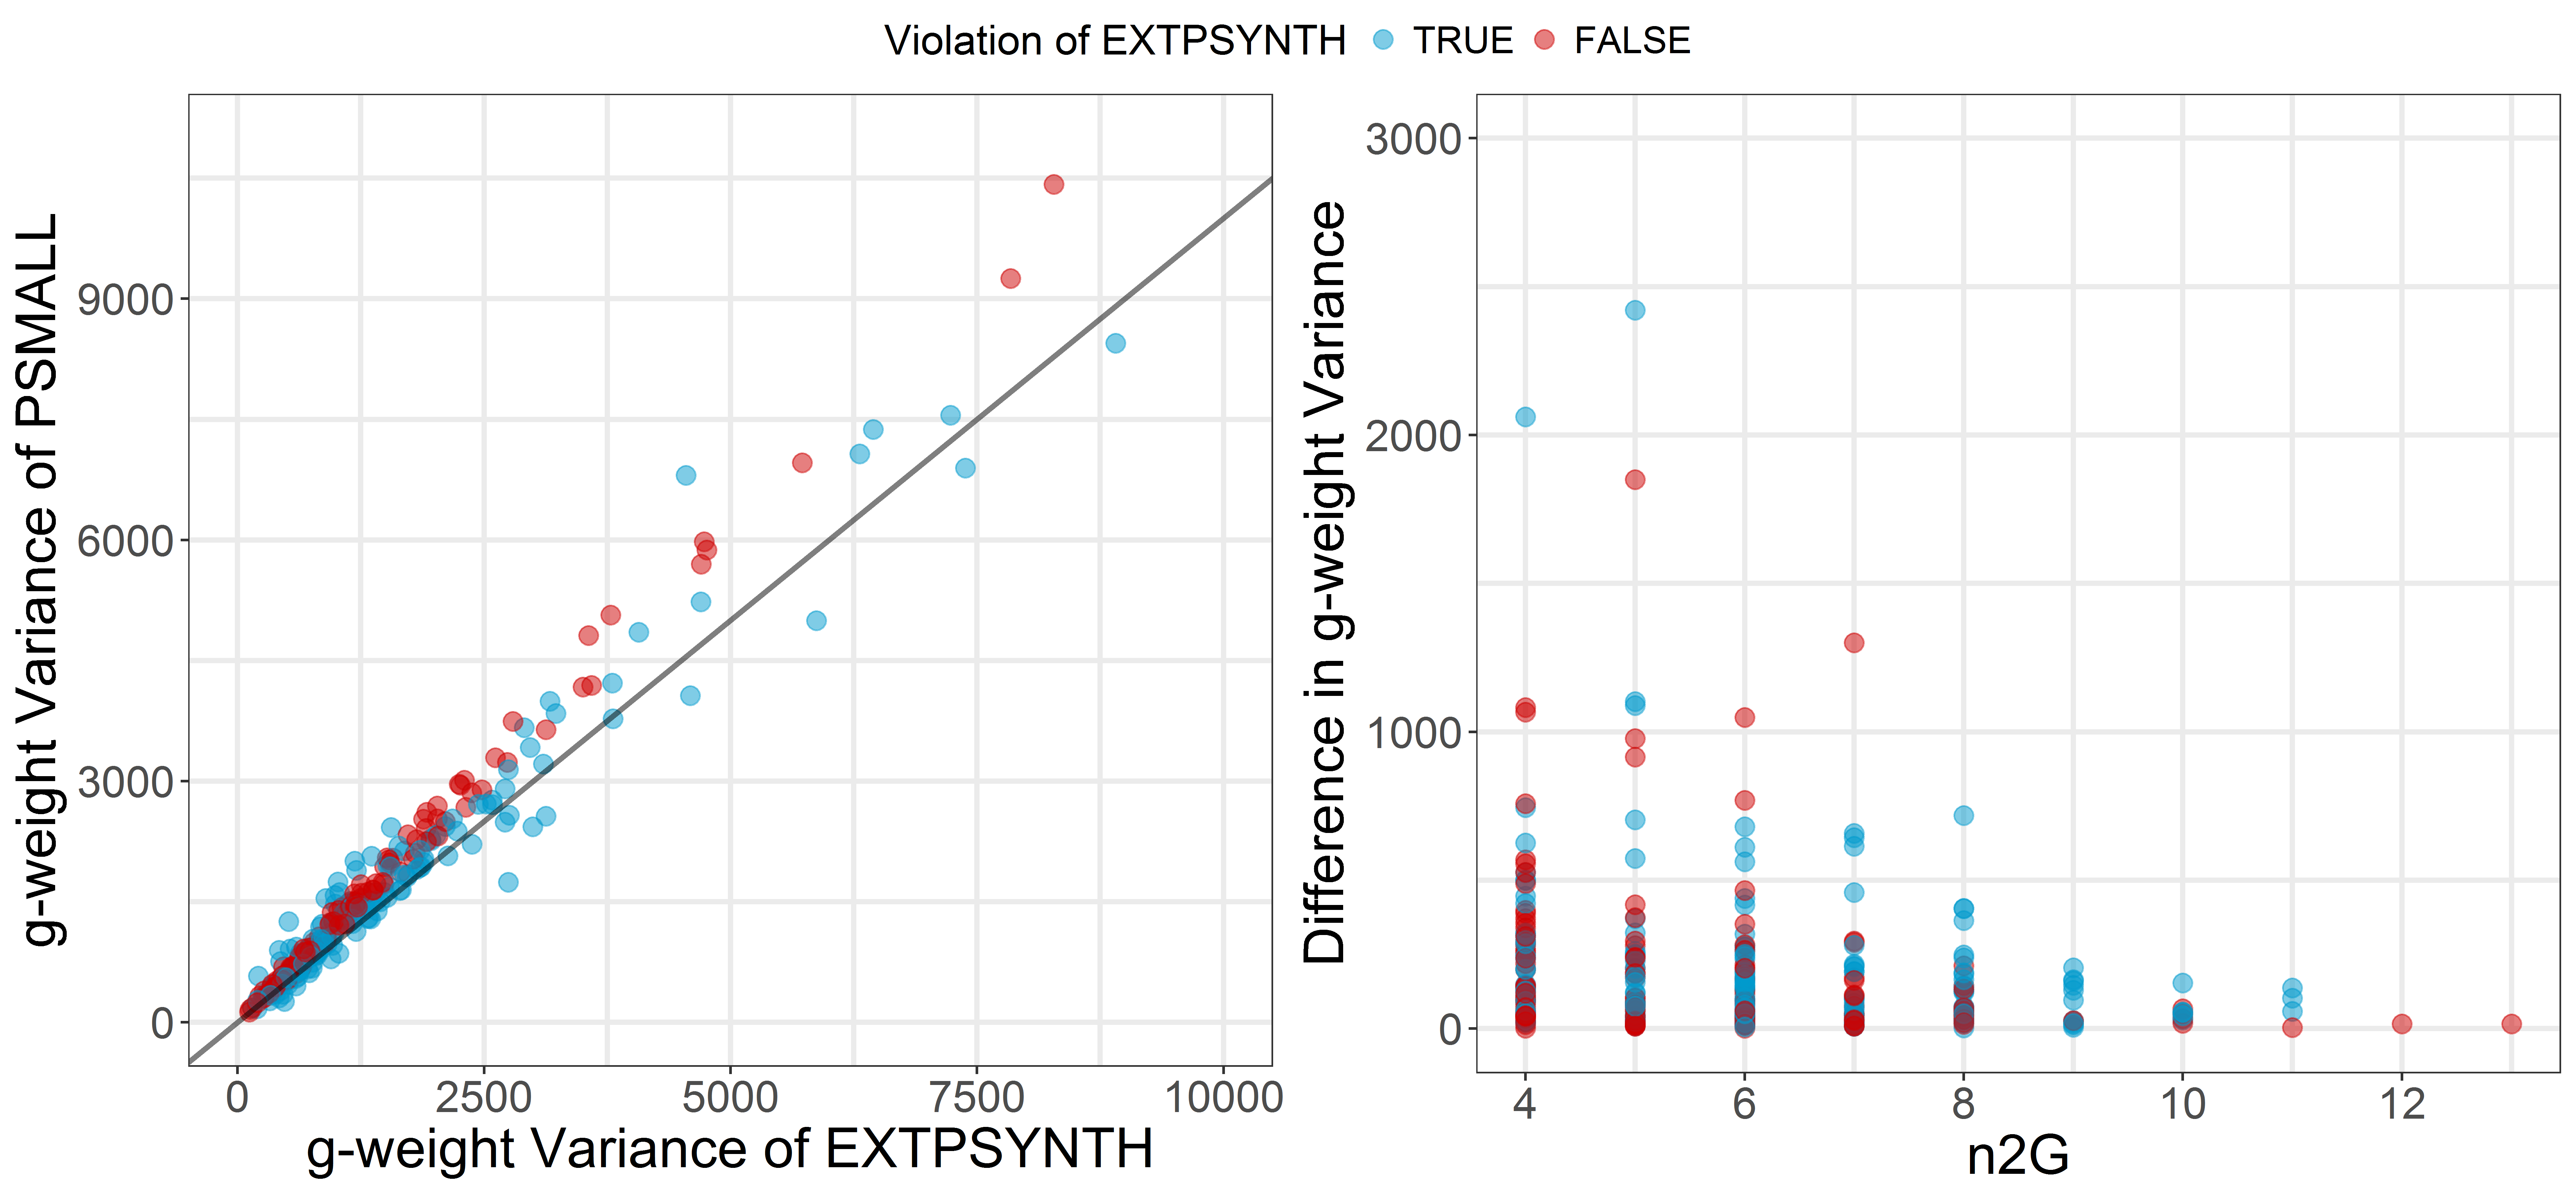
\includegraphics{fig/psmall_vs_extpsynth_fu.png}}
	\caption{\textit{Left}: Comparison of the g-weight variance between the PSMALL and the EXTPSYNTH estimator for the 321 FR units.
		\textit{Right}: Difference in g-weight variance between the PSMALL and the EXTPSYNTH estimator in dependence of the terrestrial data ($n2G$) in the FR unit.}
	\label{fig:compvar}
\end{figure}


% \newpage
% ----------------------------------------------------------------------- %
% ----------------------------------------------------------------------- %
\subsection{Reduction of SRS variance by \psmall{} and \extpsynth{}}
\label{sec:gain_eval}

We further evaluated how much the variance of the SRS estimator in each FA and FR unit was reduced by alternative application of the \psmall{} and \extpsynth{} estimator. For all FA-units, the application of \psmall{} and \extpsynth{} led to a reduction of the SRS variance that was up to 54.1\% and 49.7\% in 75\% of the FA-units (fig. \ref{fig:gain}). The differences between \psmall{} and \extpsynth{} were again due to the slightly smaller variances produced by the \extpsynth{} estimator. The reduction in variance was also expressed in the relative efficiency, which was 2.02 on average and ranged between 1.18 and 4.13 for the \extpsynth{} estimator. On FR-level, the achieved reduction in variance and the relative efficiencies reached even higher values than on FA-level (table \ref{tab:gain}). However, cases also occurred where one or both two-phase estimators produced partly substantially larger variance values than under the SRS estimator. This particularly happened in 18\% (61) of the FR-units under the \extpsynth{}, and in 23\% (76) of the FR-units under the \psmall{} estimator. 

\begin{figure}[H]
	\centering
	\resizebox{0.7\hsize}{!}{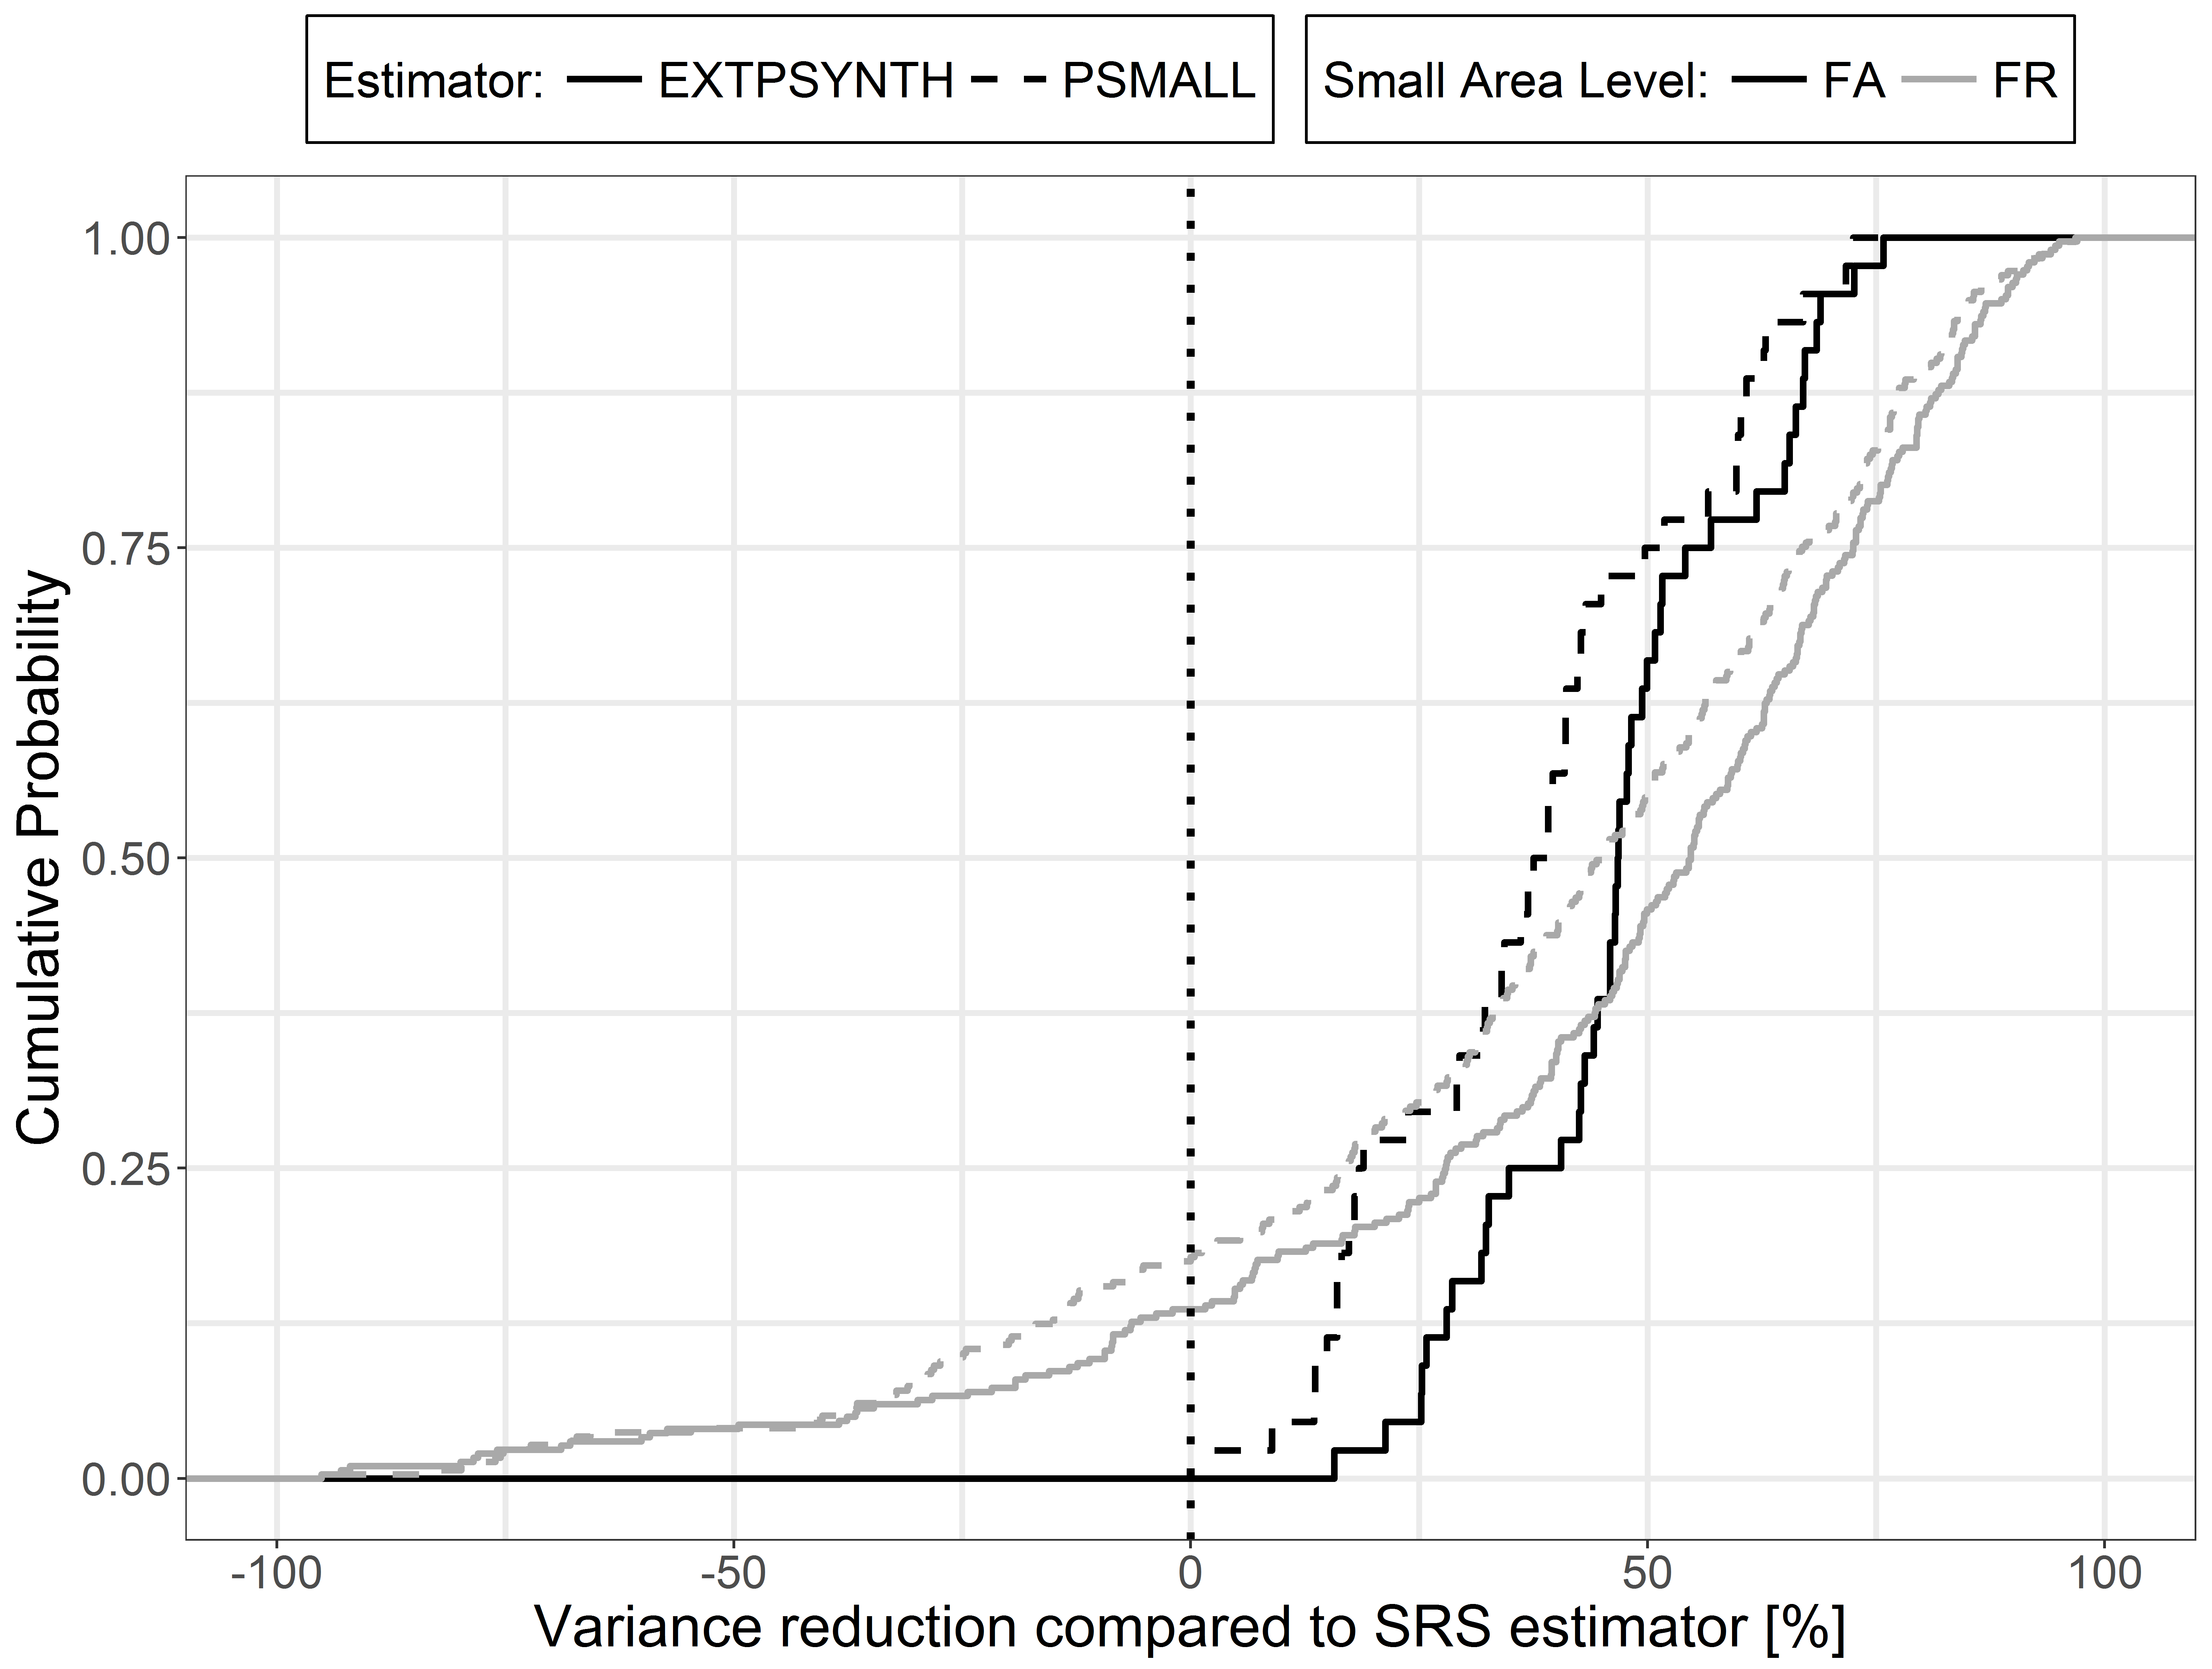
\includegraphics{fig/compare_onephase_extpsynth_psmall.png}}
	\caption{Cumulative distribution of variance reduction by the PSMALL and EXTPSYNTH compared to the SRS estimator for the  45 FA and 321 FR units.}
	\label{fig:gain}
\end{figure}


\begin{table}[H]
	\begin{center}
		\caption{Descriptive summary of SRS variance reduction and relative efficiencies on the two forest district levels. $N_u$: number of evaluated small area units.}
		\vspace{0.2cm}
		\label{tab:gain}
		{\small %
			\begin{tabular}{c|l c|c|c|c|c|c|c} %8cols
				\hlineB{1}
				\multirow{2}{*}{District level} & \multicolumn{2}{c|}{\multirow{2}{*}{Estimator}} & \multicolumn{3}{c|}{Reduction of SRS variance [\%]} & \multicolumn{3}{c}{relative efficiency} \\
				\cline{4-9} & & & mean & min & max & mean & min & max \\
				\hline \hline
				\multirow{2}{*}{FA} & PSMALL    & ($N_u$=45)  & 33.51 & 0 & 72.5 & 1.74 & 1.03 & 3.64 \\
				& EXTPSYNTH & ($N_u$=45)  & 43.30 & 0 & 75.8 & 2.03  & 1.18 & 4.13 \\
				\hlineB{2}          
				\multirow{2}{*}{FR} & PSMALL    & ($N_u$=321) & 12.48 & 0 & 96.8 & 2.54 & 0.08 & 31.61  \\
				& EXTPSYNTH & ($N_u$=321) & 24.75 & 0 & 97.0 & 2.95 & 0.10 & 33.70 \\
				\hline \hline
			\end{tabular}
		}%
	\end{center}
\end{table}

Here comes some detective work ...





\begin{figure}[H]
	\centering
	\resizebox{0.7\hsize}{!}{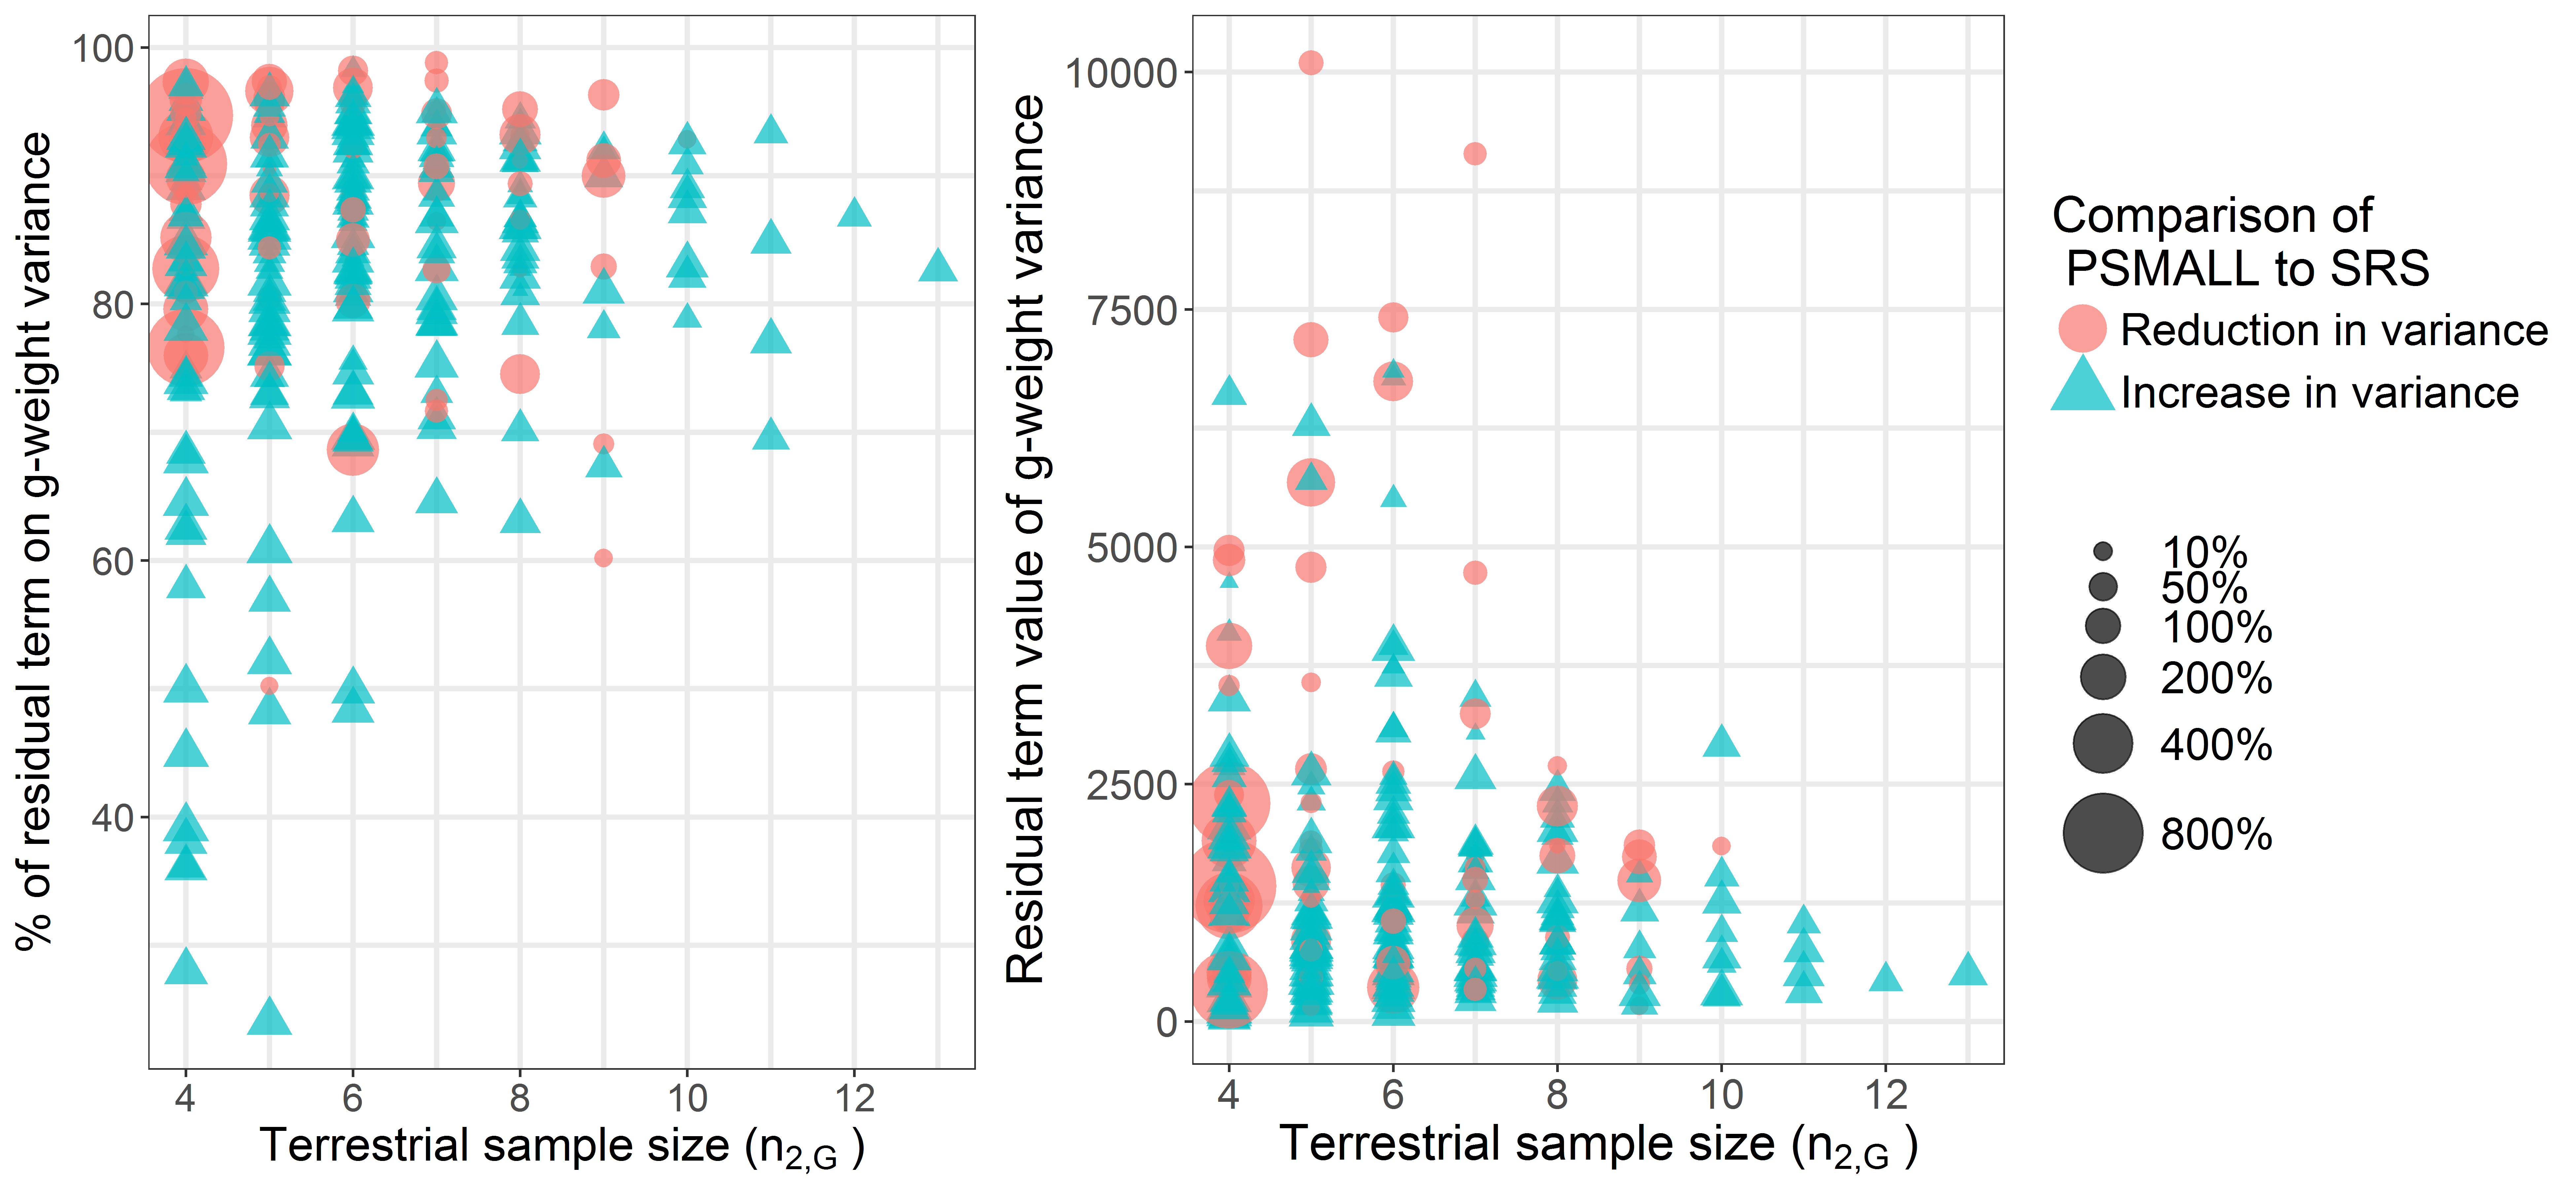
\includegraphics{fig/eval_2phase_fail.png}}
	\caption{}
	\label{fig:fail}
\end{figure}










